\documentclass[UTF-8]{article}
\usepackage{amsmath}
\usepackage{amssymb}
\usepackage{float}
\usepackage{graphicx}
\usepackage{epstopdf}
\usepackage{inputenc}
\usepackage{geometry}
\usepackage{pgfplots} 
\usepackage{listings}
\usepackage{color}
\geometry{left=2.5cm,right=2.5cm,top=2.5cm,bottom=2.5cm}

\definecolor{codegreen}{rgb}{0,0.6,0}
\definecolor{codegray}{rgb}{0.5,0.5,0.5}
\definecolor{codepurple}{rgb}{0.58,0,0.82}
\definecolor{backcolour}{rgb}{0.9,0.9,0.92}

\lstdefinestyle{mystyle}{
	backgroundcolor=\color{backcolour},   
	commentstyle=\color{codegreen},
	keywordstyle=\color{blue},
	numberstyle=\tiny\color{codegray},
	stringstyle=\color{codepurple},
	basicstyle=\ttfamily\footnotesize,
	breakatwhitespace=false,         
	breaklines=true,                 
	captionpos=b,                    
	keepspaces=true,                 
	numbers=left,                    
	numbersep=5pt,                  
	showspaces=false,                
	showstringspaces=false,
	showtabs=false,                  
	tabsize=2
}

\lstset{style=mystyle}


\title{VU Computer Vision 2023 \\
	\large Assignment 1} %exchange for assignment number

\author{Sebastian Bergner}
\begin{document}
	
	\maketitle
	
	\section*{Task 1}
	(0.5 points) Install OpenCV\\
	
	\begin{lstlisting}[language=bash]
pip3 install opencv-python
pip3 install opencv-contrib-python #for the full package incl extra modules\end{lstlisting}
Optionally you could set up a virtual environment (\verb|python3 -m venv venv|).

\section*{Task 2}
(0.5 points) Take a picture with your smartphone, resize the picture as to be 448x336 pixels.
	
\begin{figure}[H]
	\centering
	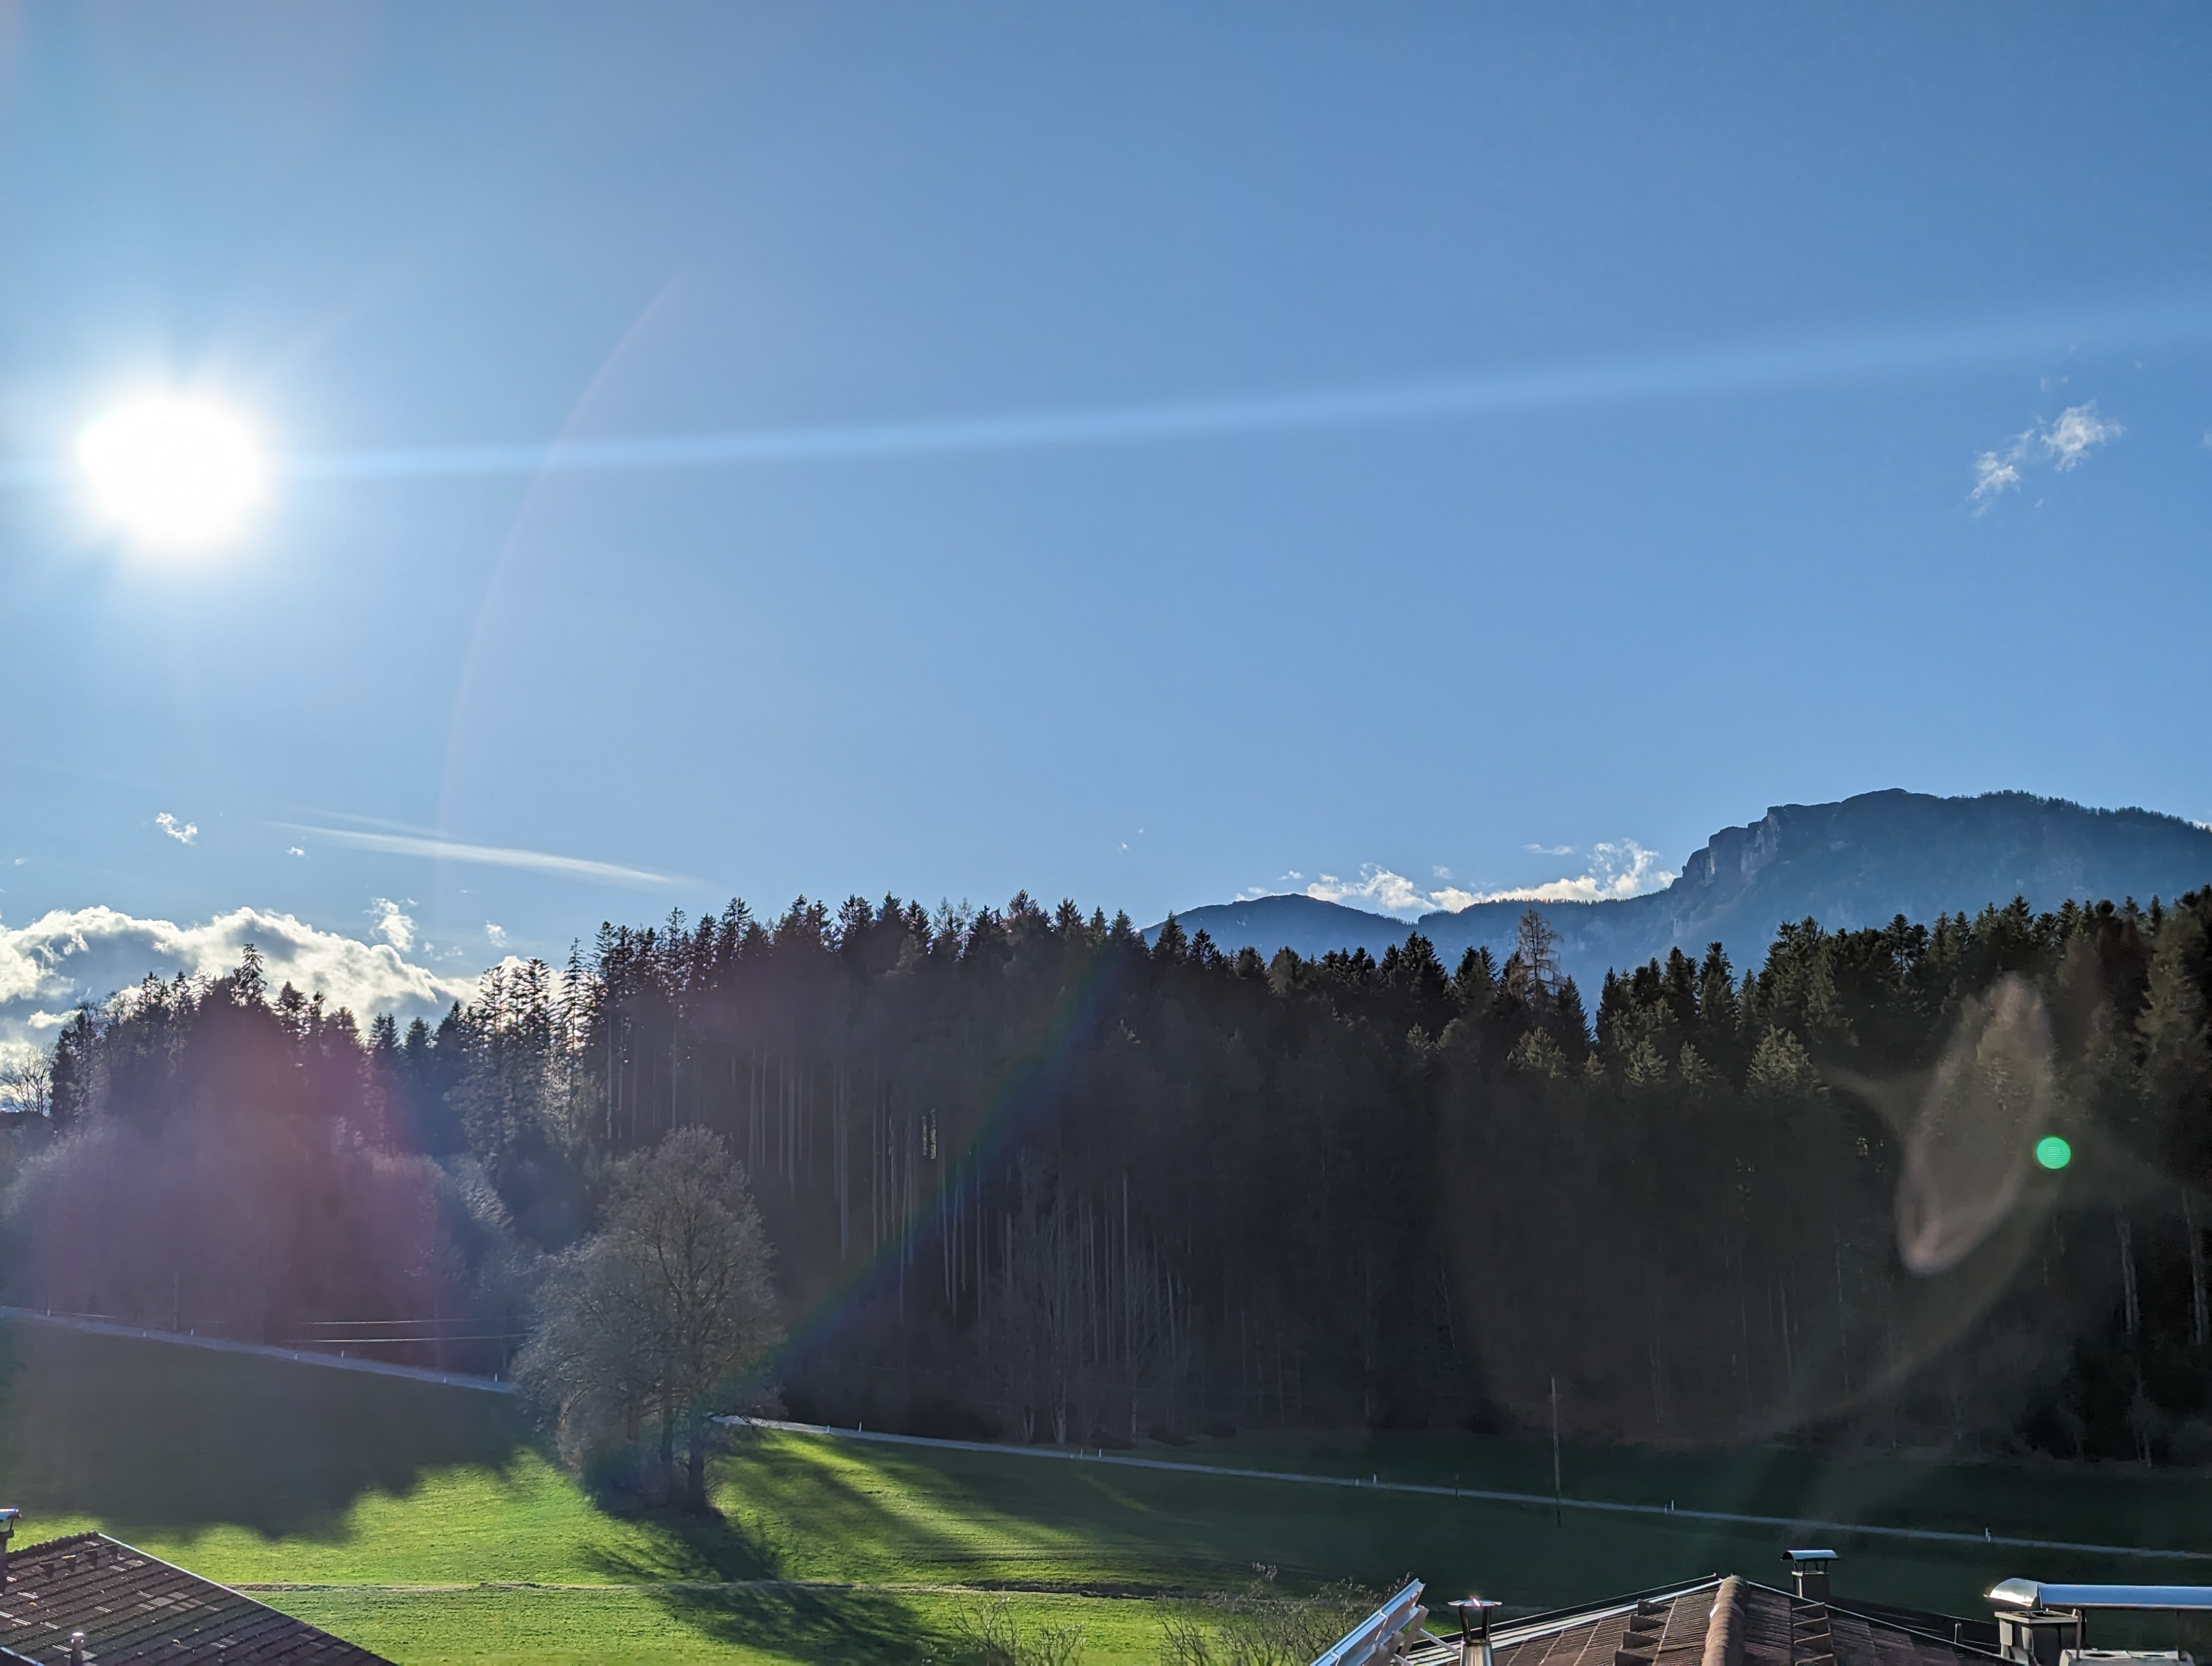
\includegraphics[scale=0.1]{photo}
	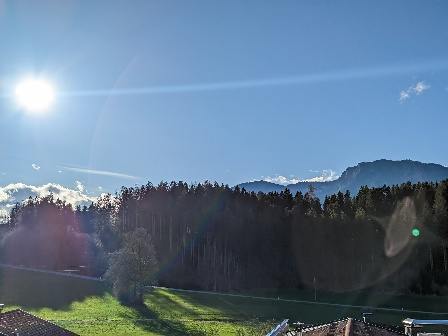
\includegraphics[scale=0.1]{resized_photo}
	\caption{Photo and resized photo. (Both scaled down to 10\%)}
	\label{fig:resizedphoto}
\end{figure}



\begin{lstlisting}
import cv2 as cv

im = cv.imread('photo.jpg', cv.IMREAD_UNCHANGED)

resized_im = cv.resize(im, (448, 336), interpolation=cv.INTER_CUBIC)
cv.imwrite('resized_photo.jpg', resized_im)

cv.imshow('resized image', resized_im)
cv.waitKey(0)
cv.destroyAllWindows()
\end{lstlisting}

There are several interpolation types/algorithms available like linear or bicubic, I decided to use the inter\_cubic. There won't be such a strong difference between the types at least not visible without any tools.
\newpage
\section*{Task 3}
(2 points) Apply a Gabor filter at 4 orientations. What are the differences you note among the
4 orientations? Combine the 4 orientations (max or sum), what do you see.
\begin{figure}[H]
	\centering
	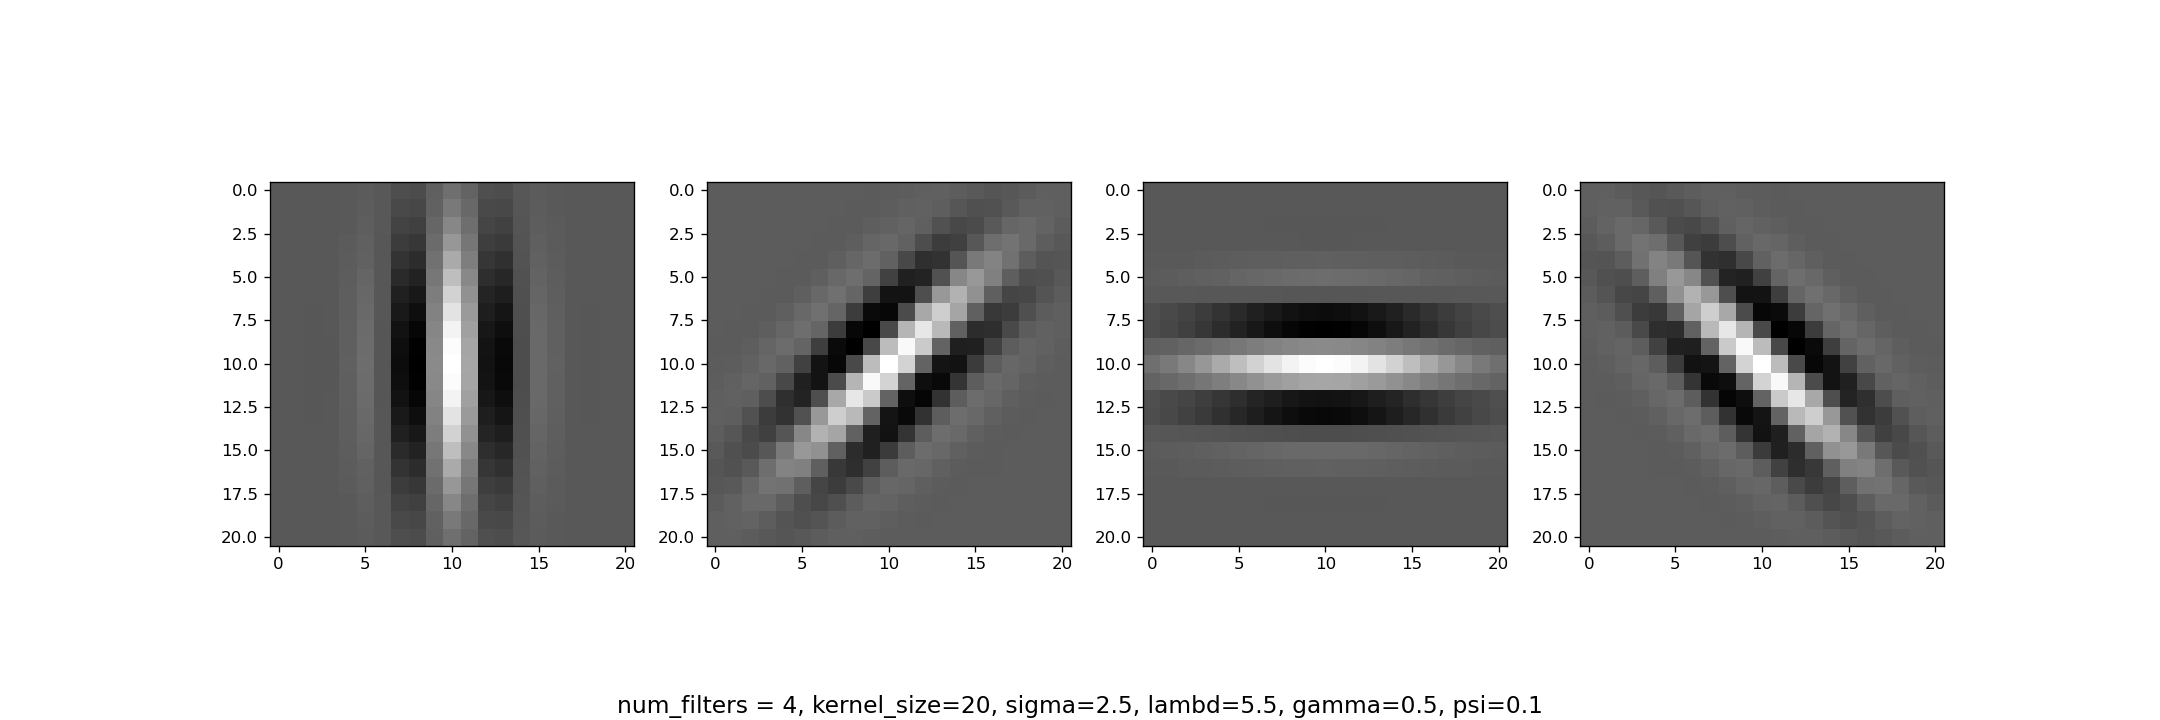
\includegraphics[width=0.7\linewidth]{gabor1}
	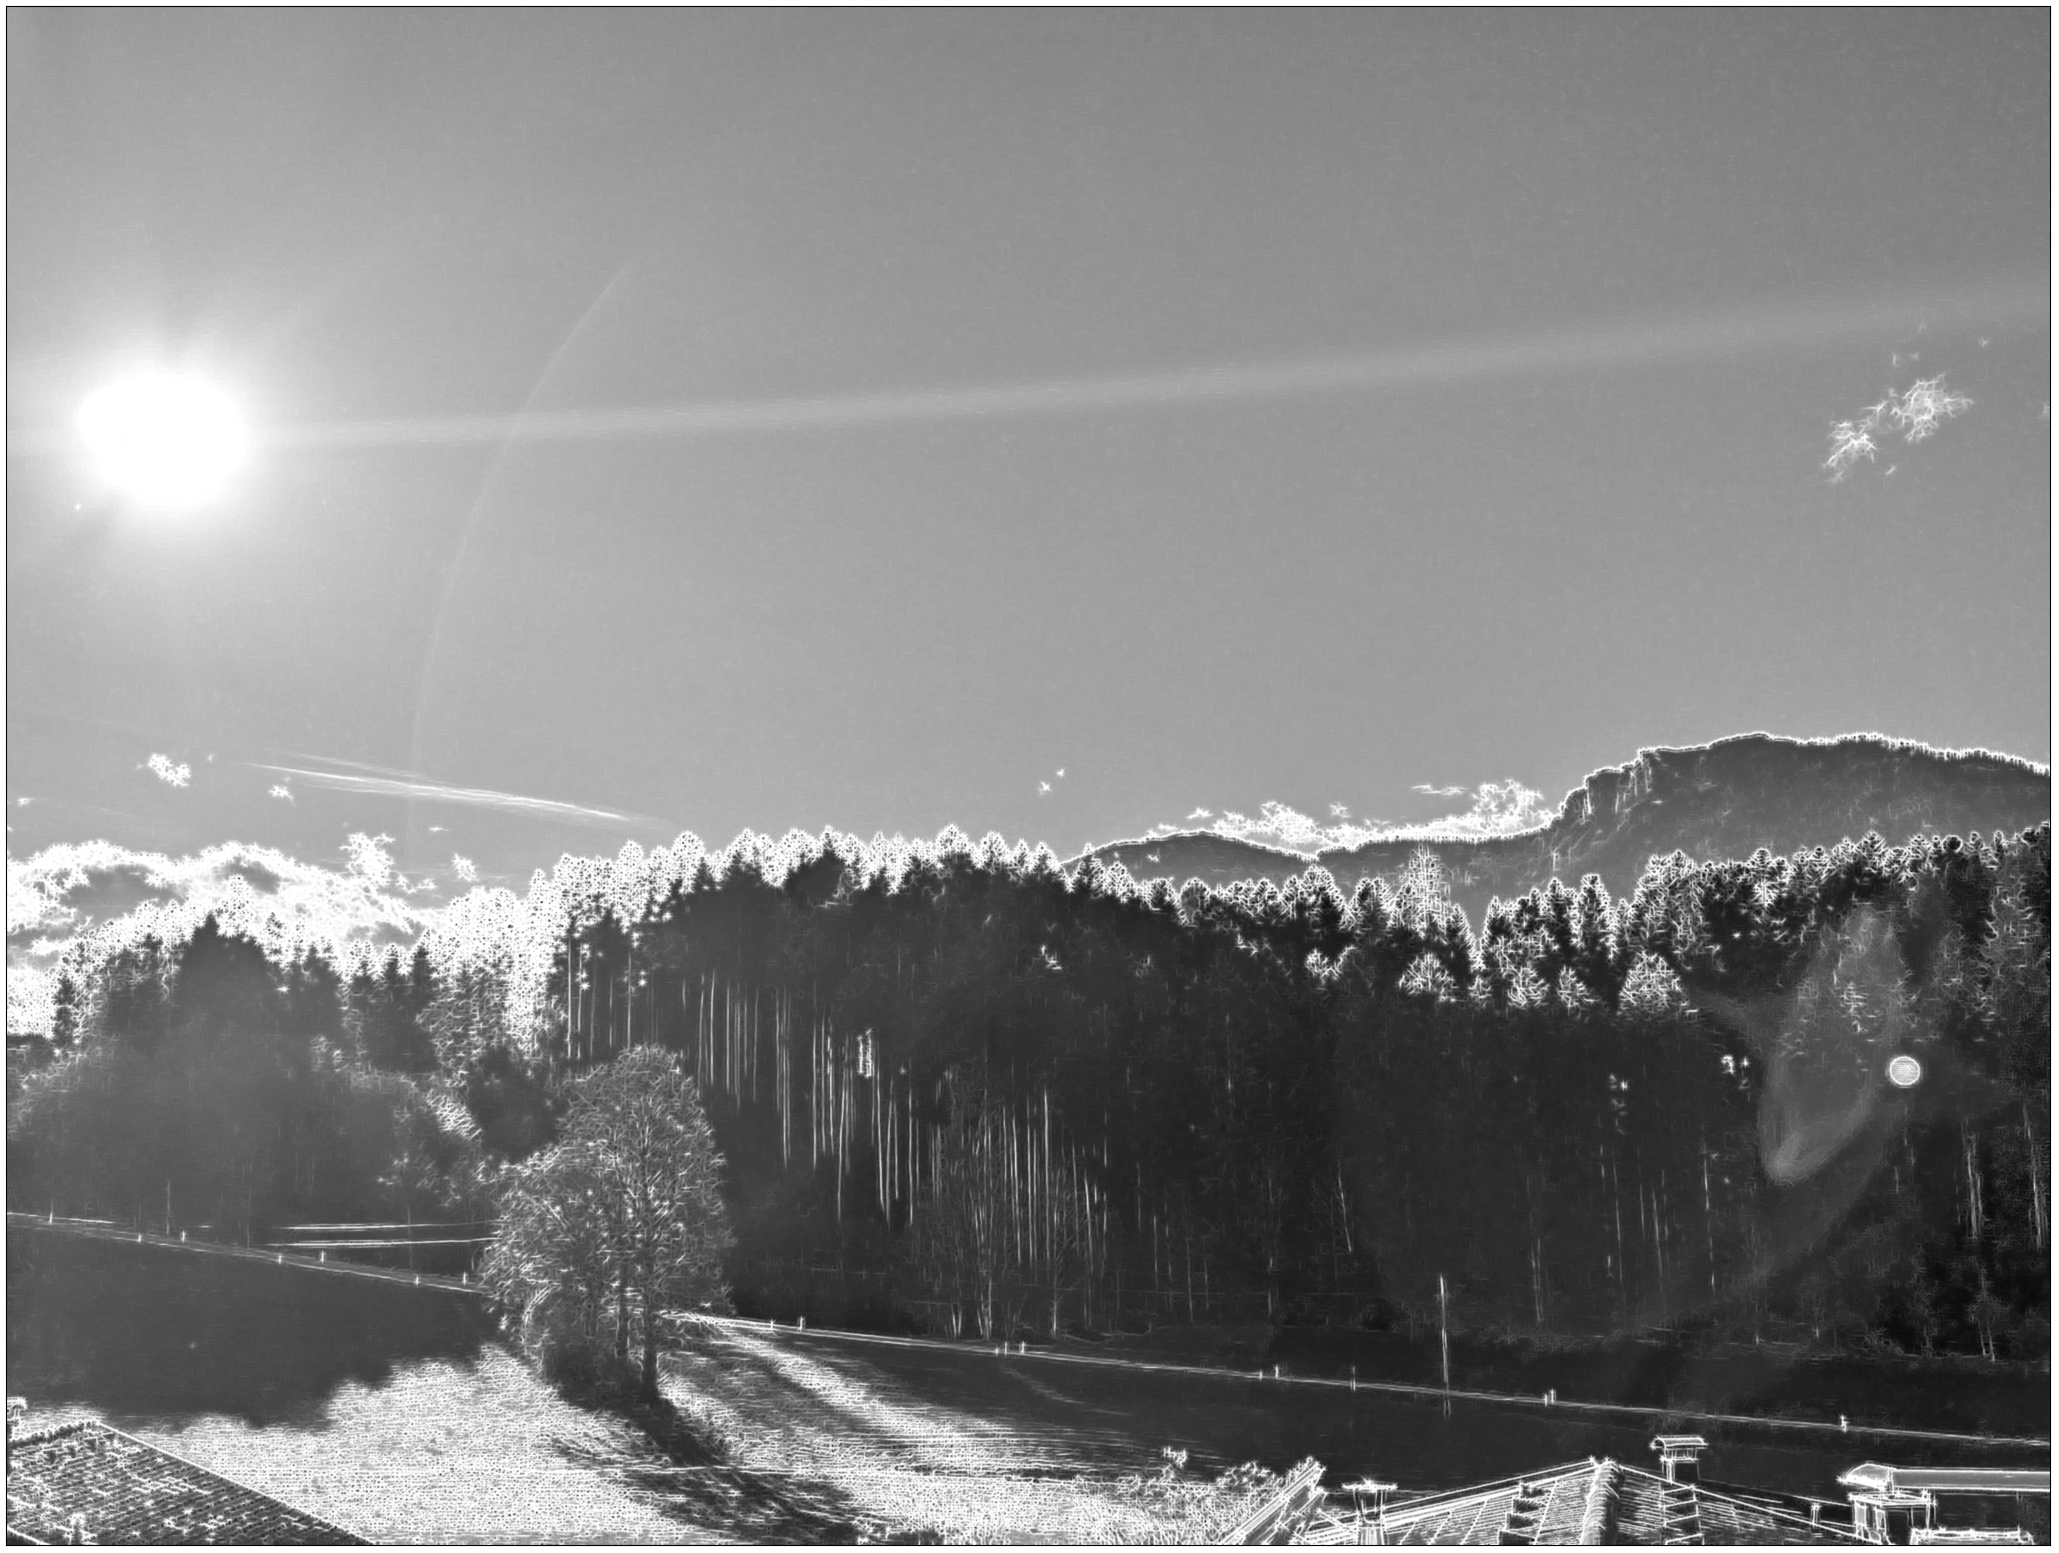
\includegraphics[width=0.7\linewidth]{gabor2}
	\caption{Gabor filters and image with filters.}
	\label{fig:gabor1}
\end{figure}

\begin{figure}[H]
	\centering
	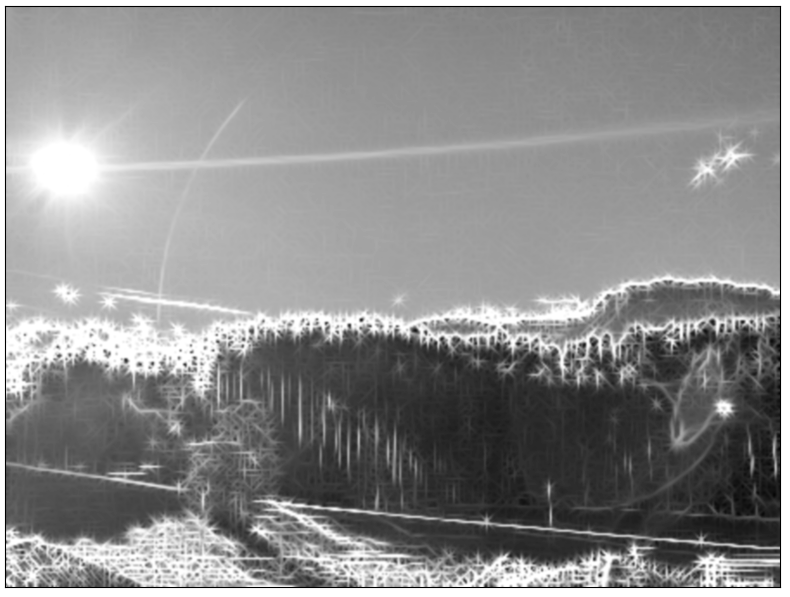
\includegraphics[width=0.7\linewidth, scale=1.1]{gabor3}
	\caption{Resized image with applied filter.}
	\label{fig:gabor2}
\end{figure}

Using the gabor filter, all the edges are highlighted. Edges with the same direction as one of the filters should be highlighted more intensely than the other ones.
\\
In the second figure the gabor filters with its effects are much more pronounced than in the original one. This is due to the size of the kernel in relation to the image.

\begin{lstlisting}[language=python]
import cv2 as cv
import numpy as np
import helpers

im = cv.imread('resized_photo.jpg', cv.IMREAD_GRAYSCALE)

def create_filter(num_filters=4, kernel_size=35, sigma=1.5, lambd=3.5, gamma=0.5, psi=0.1):
	filters = []
	for theta in np.arange(0, np.pi, np.pi / num_filters):
		kern = cv.getGaborKernel((kernel_size, kernel_size), sigma, theta, lambd, gamma, psi, ktype=cv.CV_64F)
		kern /= 1.0 * kern.sum()
		filters.append(kern)
	return filters

def apply_filter(img, filters):
	newimage = np.zeros_like(img)
	for kern in filters:
		image_filter = cv.filter2D(img, -1, kern)
		np.maximum(newimage, image_filter, newimage)
	return newimage

gfilters = create_filter()
image_g = apply_filter(im, gfilters)


helpers.showimages(gfilters, (18, 6))
helpers.showimage(image_g)\end{lstlisting}


\newpage
\section*{Task 4}
(1.5 points) Play with the parameters of the filter and show how the filter works with 3 different
parameter values.

The code is the same as in previous task. Only the function parameters are varied.

Changing only $\sigma$ seems to change the width of the filter. Applied it seems to affect the threshold which is assumed as there are many more artifacts in midair.

\begin{figure}[H]
	\centering
	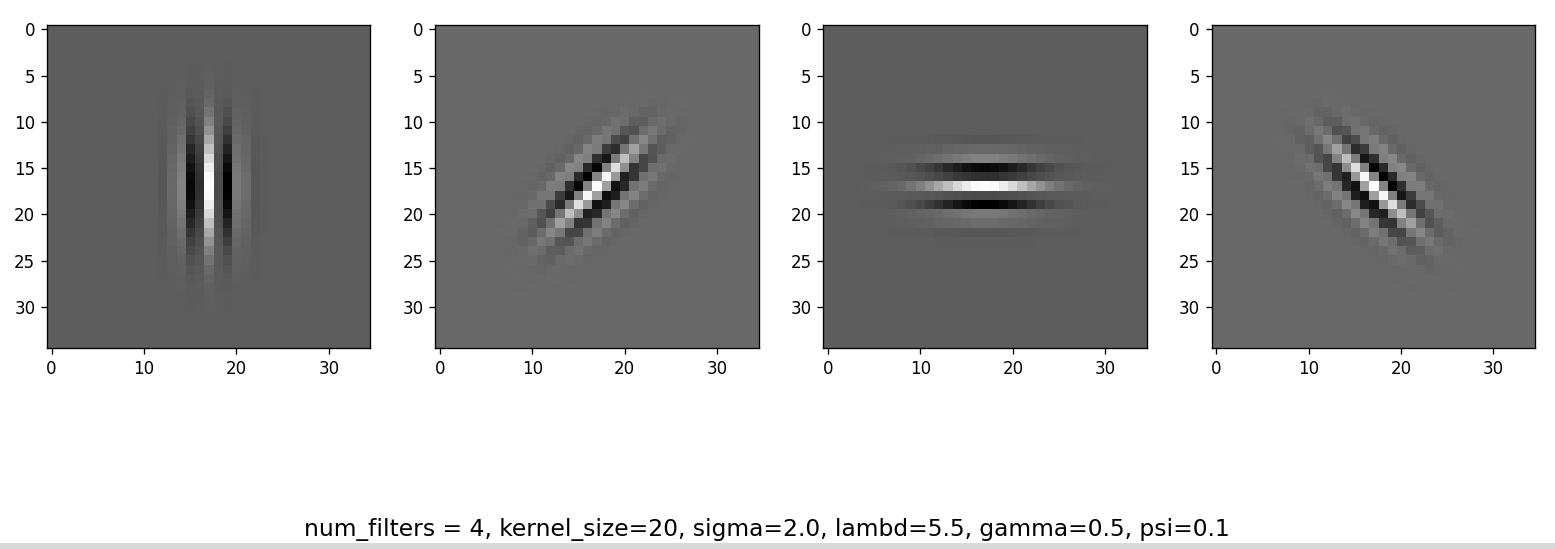
\includegraphics[width=0.7\linewidth]{task4_1}
	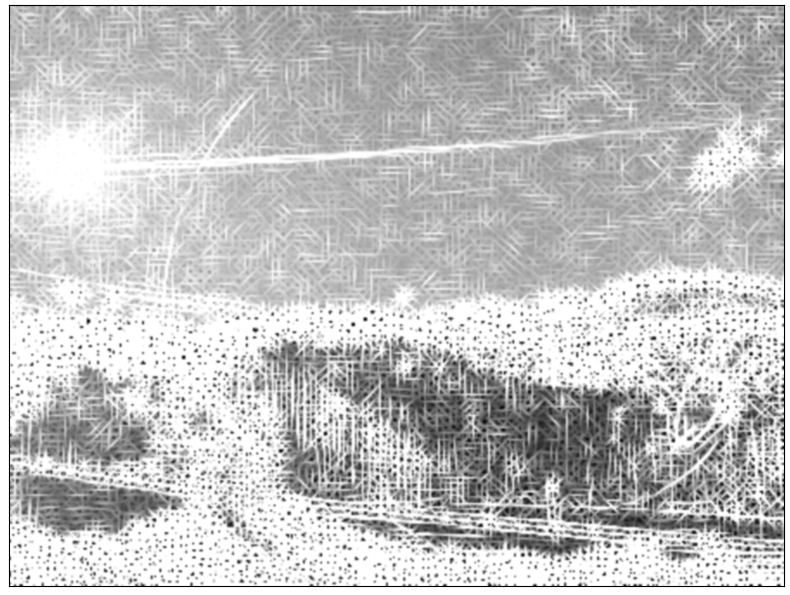
\includegraphics[width=0.7\linewidth]{task4_2}
	\caption{$\sigma = 2.0$}
	\label{fig:task41}
\end{figure}
\newpage

Increasing $\lambda$ seems to cut off lower values of the filter leaving only the highest perturbation. Applied to the image yields a quite unsharp image with actually very few signs of the filter.

\begin{figure}[H]
	\centering
	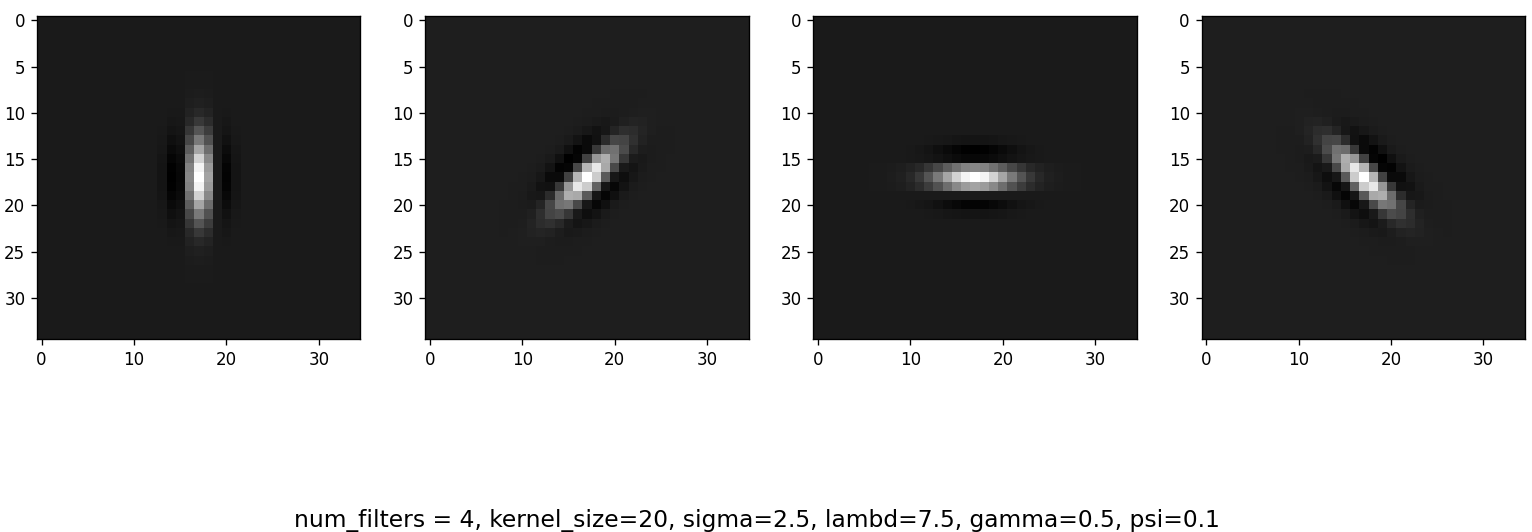
\includegraphics[width=0.7\linewidth]{task4_3}
	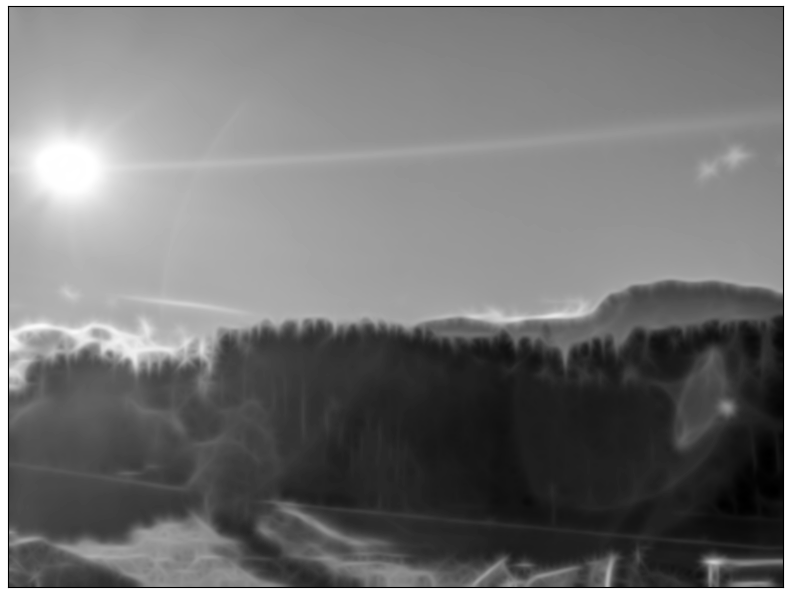
\includegraphics[width=0.7\linewidth]{task4_4}
	\caption{$\lambda = 7.5$}
	\label{fig:task42}
\end{figure}
\newpage
Changing $\gamma$ to a greater value seems to bound the filter to a smaller size this can be well observed in the image below. Here the individual applications seem more bound to edges.

\begin{figure}[H]
	\centering
	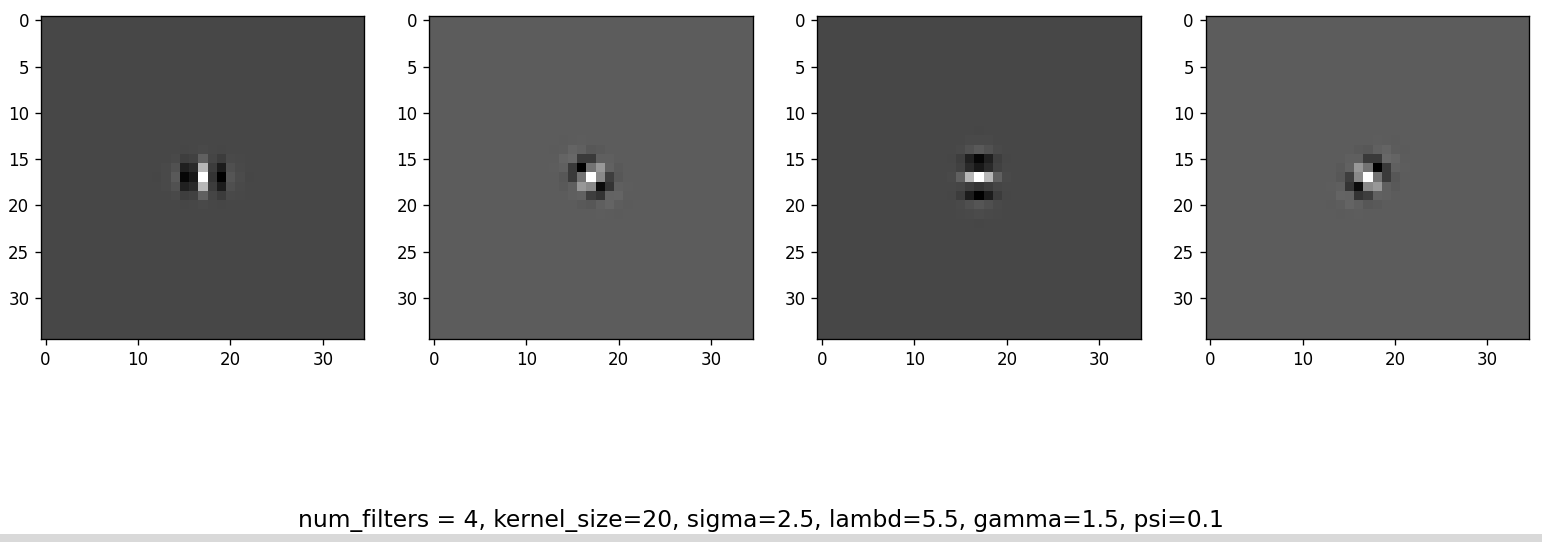
\includegraphics[width=0.7\linewidth]{task4_5}
	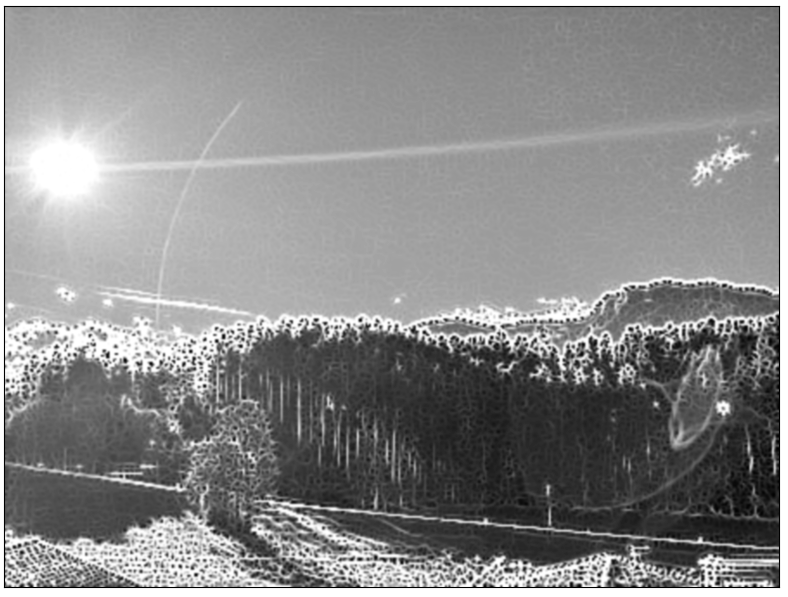
\includegraphics[width=0.7\linewidth]{task4_6}
	\caption{$\gamma = 1.5$}
	\label{fig:task43}
\end{figure}
\newpage
Increasing $\psi$ seems to increase the filters value, like a offset. This yields a similar image as like the first one but with less pronunciation of the single "activations".

\begin{figure}[H]
	\centering
	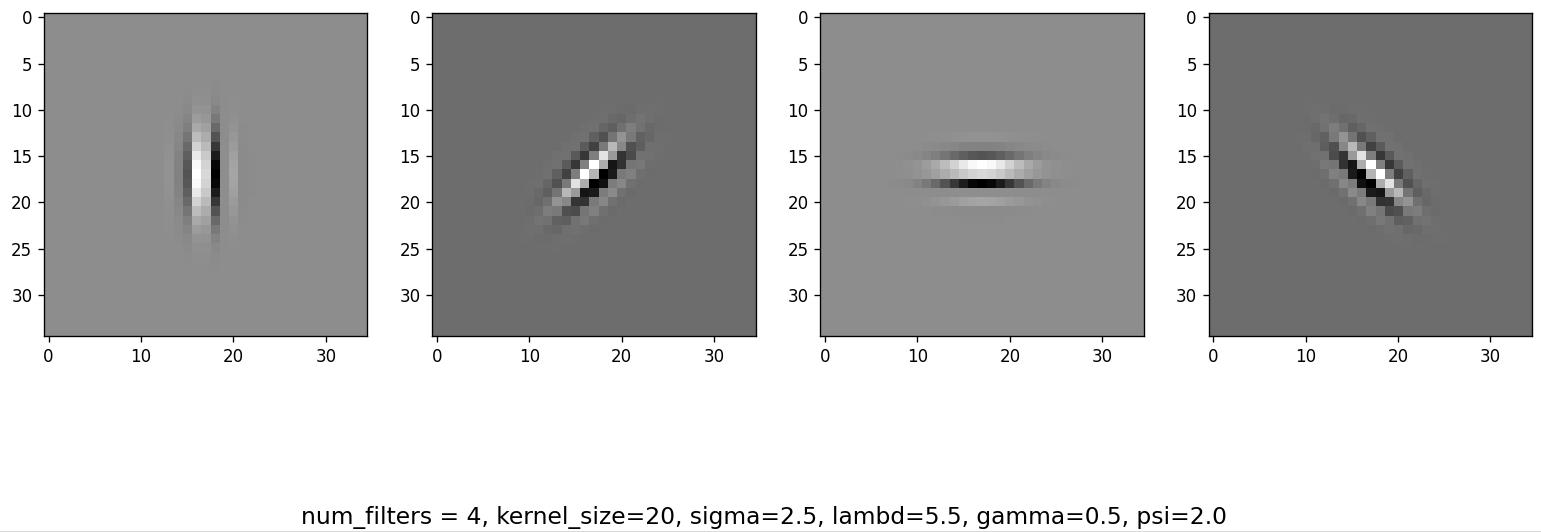
\includegraphics[width=0.7\linewidth]{task4_7}
	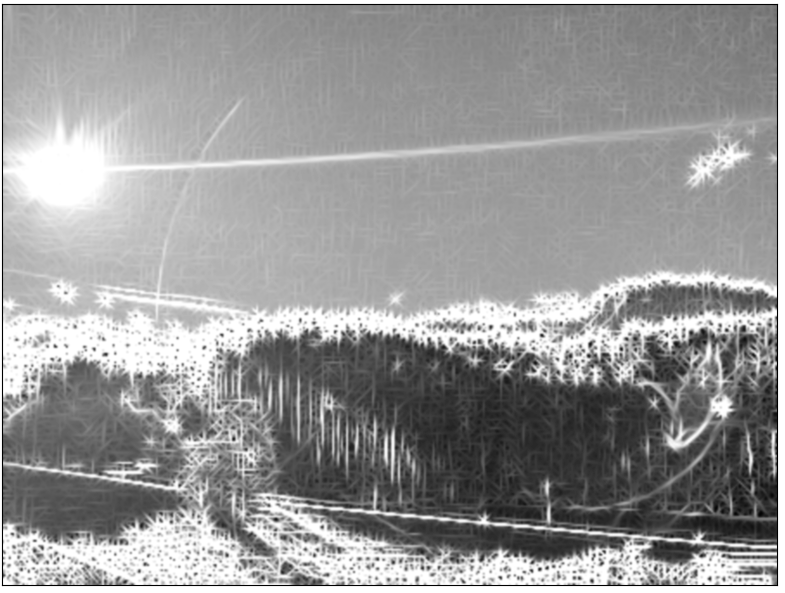
\includegraphics[width=0.7\linewidth]{task4_8}
	\caption{$\psi = 2.0$}
	\label{fig:task44}
\end{figure}
\newpage

\section*{Task 5}
(2 points) Implement a Gaussian Pyramid. Show the results using the same image. Comment
on the results. What are the low frequencies?

The low frequencies would correnspond in this image to the sky and the sun. This is visible when comparing the first image with the last where all the high frequencies are smoothed away such as the noise or here when zooming in the texture of the forest itself. The forest for example is just a mostly black uniform part of the last image, where in the first one (in this grayscaled version) at least the tree crowns and their branches are distinguishable.

\begin{figure}[H]
	\centering
	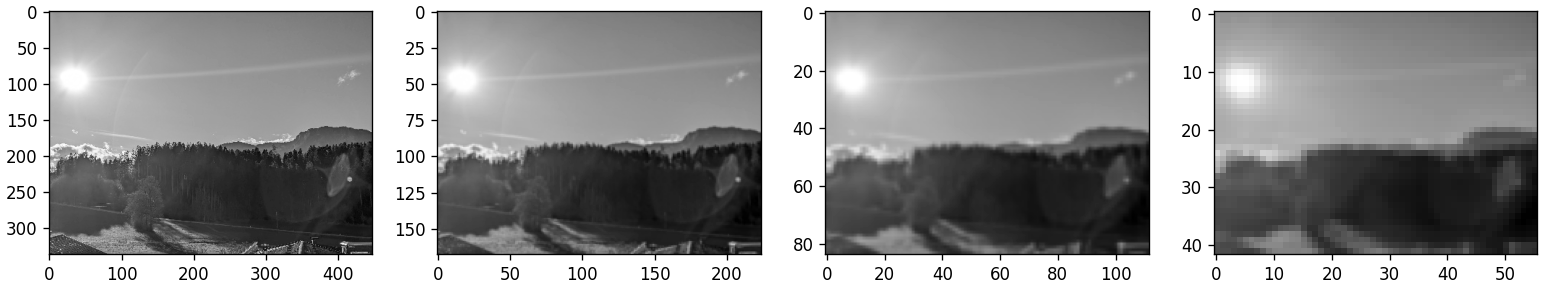
\includegraphics[width=1\linewidth]{gaussian}
	\caption{Gaussian pyramid of the resized image.}
	\label{fig:gaussian}
\end{figure}

\begin{figure}[H]
	\centering
	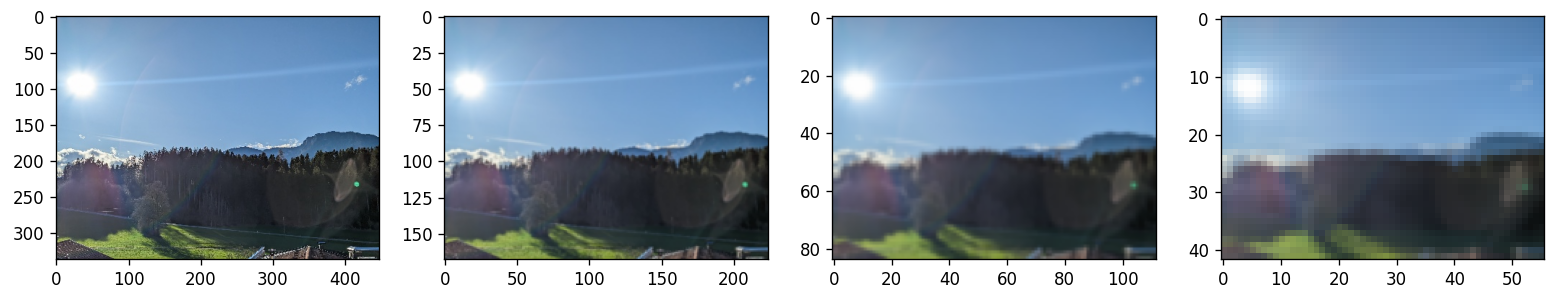
\includegraphics[width=1\linewidth]{gaussian_color.png}
	\caption{Gaussian pyramid of the resized image in color.}
	\label{fig:gaussian2}
\end{figure}

\begin{lstlisting}[language=python]
import cv2
import helpers

img = cv2.imread("resized_photo.jpg", cv2.IMREAD_GRAYSCALE)
helpers.showimage(img)

images = list()
images.append(img)
for i in range(4):
	images.append(cv2.pyrDown(images[i]))

helpers.showimages(images, (18,6))
\end{lstlisting}
\newpage
\section*{Task 6}
(1.5 points) Create a Laplacian Pyramid using the code from (5). Show the pyramid and
comment on the results.
\\
The laplacian pyramid shows the difference of a step in a gaussian pyramid. So a laplacian pyramid can be used to visualize high frequency areas in a image with an even greater distinction than a gaussian. The white (or color in case of a colored gaussian pyramid) areas in the below images are the high frequency areas. The images from left to right show the highest frequencies and are stepping down from highest to lowest. Also the edges get broader.
\begin{figure}[H]
	\centering
	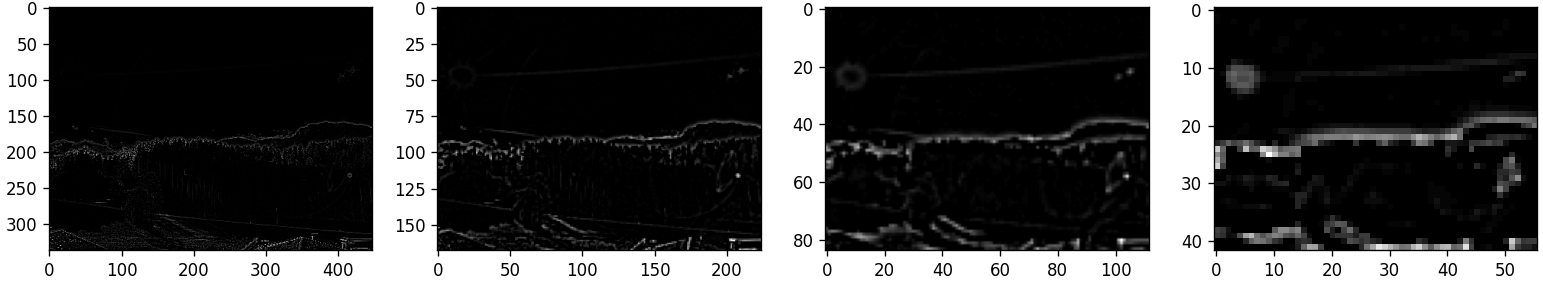
\includegraphics[width=1\linewidth]{laplacian}
	\caption{Laplacian pyramid of the resized image.}
	\label{fig:laplacian}
\end{figure}

\begin{lstlisting}[language=python]
import cv2
from matplotlib import pyplot as plt
import helpers

img = cv2.imread("resized_photo.jpg", cv2.IMREAD_GRAYSCALE)
helpers.showimage(img)
#gaussian
images = list()
images.append(img)
for i in range(4):
	images.append(cv2.pyrDown(images[i]))

helpers.showimages(images, (18,6))
#laplacian
laplacian_images = list()

for i in range(4):
	laplacian_images.append(cv2.subtract(images[i], cv2.pyrUp(images[i+1])))

helpers.showimages(laplacian_images, (18,6))
cv2.waitKey()
\end{lstlisting}

\section*{Task 7}
(2 points) Apply the Fourier transform and provide the magnitude and phase images.
The two figures below show images of the optimized image, magnitude and phase. The first one is based on the full resolution original photo and the second one shows the resized one. Interestingly the lower one shows some interesting artifacts on both phase and magnitude. For visualization of the fourier transform the quadrants have been swapped in the same manner as the original one.
	
\begin{figure}[H]
	\centering
	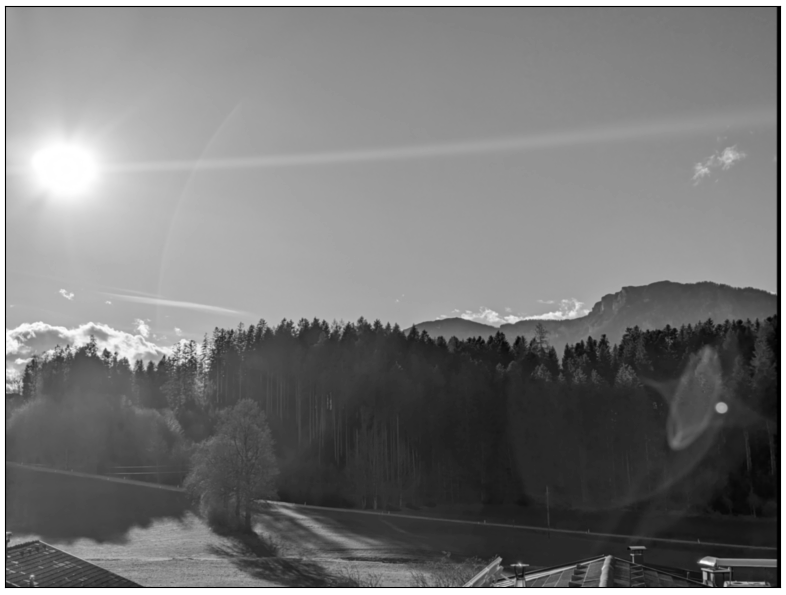
\includegraphics[width=0.5\linewidth]{fourier_orig_with_border}
	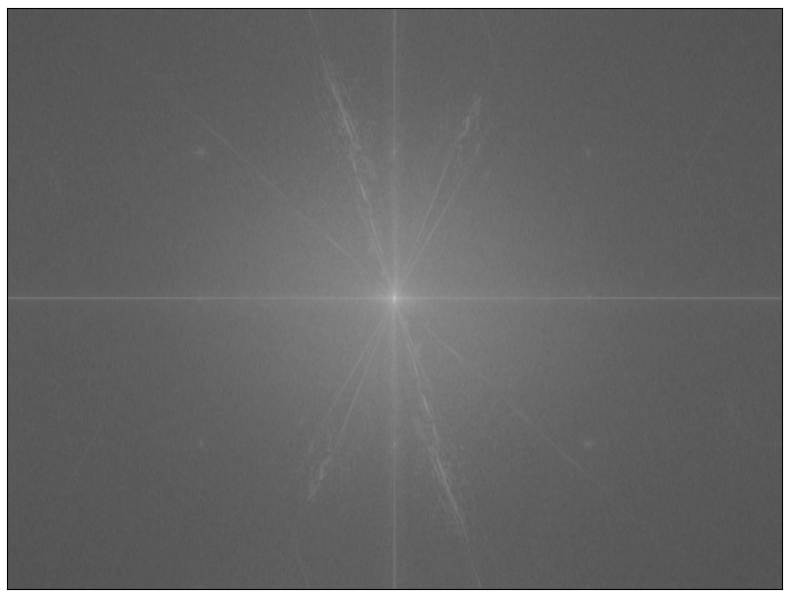
\includegraphics[width=0.5\linewidth]{fourier_orig_magnitude.png}
	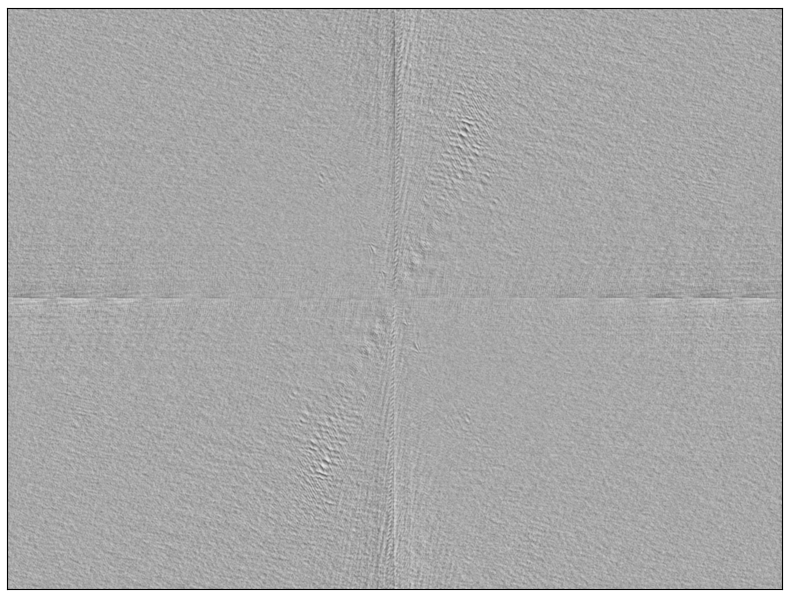
\includegraphics[width=0.5\linewidth]{fourier_orig_phase.png}
	\caption{Fourier transform on the original photo. 1. optimized image 2. magnitude 3. phase}
	\label{fig:fourierorigwithborder}
\end{figure}

\begin{figure}[H]
	\centering
	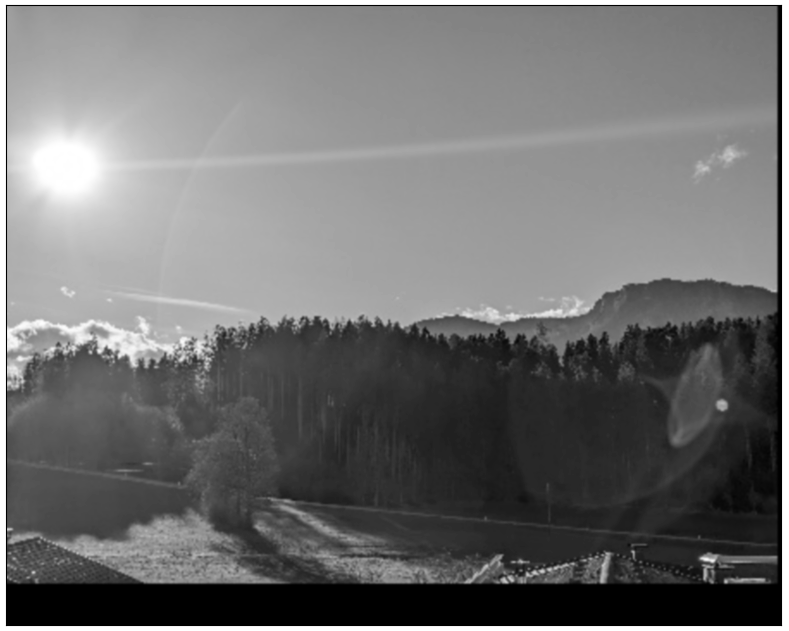
\includegraphics[width=0.5\linewidth]{fourier_resized_with_border.png}
	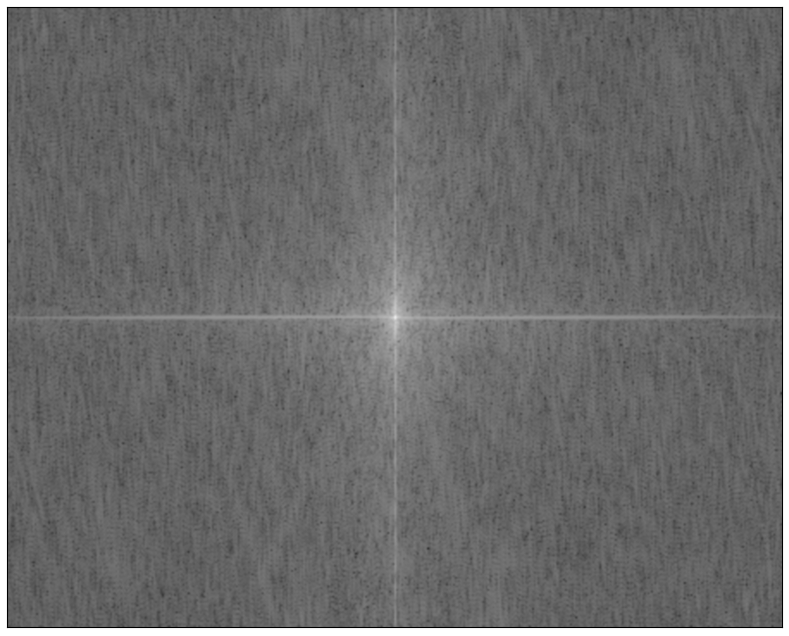
\includegraphics[width=0.5\linewidth]{fourier_resized_magnitude.png}
	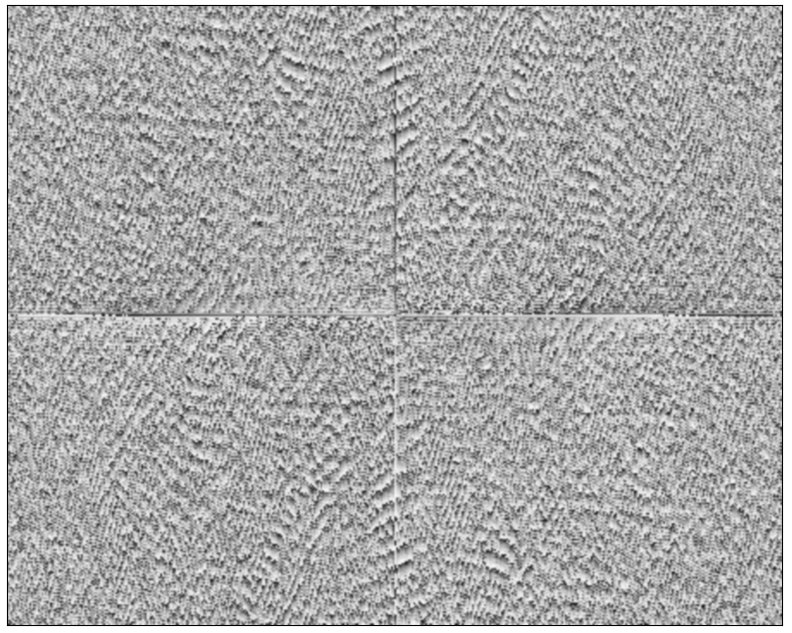
\includegraphics[width=0.5\linewidth]{fourier_resized_phase.png}
	\caption{Fourier transform on the original photo. 1. optimized image 2. magnitude 3. phase}
	\label{fig:fourierscaledwithborder}
\end{figure}
\newpage
\begin{lstlisting}[language=python]
import helpers
import cv2 as cv
import numpy as np

im = cv.imread('photo.jpg', cv.IMREAD_GRAYSCALE)

m = cv.getOptimalDFTSize(im.shape[0])
n = cv.getOptimalDFTSize(im.shape[1])

#add border to make img optimal for discrete fourier
im_border = cv.copyMakeBorder(im, 0, m-im.shape[0], 0, n-im.shape[1], cv.BORDER_CONSTANT, None, 0)

#show image with the added border
helpers.showimage(im_border)

#generate array to store the generated img
planes = np.array([np.copy(im_border), np.zeros(im_border.shape, np.float32)])

complexI = cv.merge(planes)
complexI = cv.dft(complexI)

cv.split(complexI, planes)

magI = cv.magnitude(planes[0], planes[1])
magI += 1.0
magI = cv.log(magI)
magI = magI[0:(magI.shape[0] & -2), 0:(magI.shape[1] & -2)]
helpers.swap_quadrants(magI)
magI = cv.normalize(magI, None, 0, 1, cv.NORM_MINMAX)
helpers.showimage(magI)

phase = cv.phase(planes[0], planes[1])
phase += 1.0
phase = cv.log(phase)
phase = phase[0:(phase.shape[0] & -2), 0:(phase.shape[1] & -2)]
helpers.swap_quadrants(phase)
phase = cv.normalize(phase, None, 0, 1, cv.NORM_MINMAX)
helpers.showimage(phase)
\end{lstlisting}


\section*{Appendix}
To make the code more readable and remove redundancies I've added a small helper class with some useful functions. Below is the file.

\begin{lstlisting}[language=python]
import cv2
import numpy as np
from matplotlib import pyplot as plt


def showimage(myimage, figsize=[10,10]):
	if (myimage.ndim>2):
		myimage = myimage[:,:,::-1]
	_, ax = plt.subplots(figsize=figsize)
	ax.imshow(myimage, cmap = 'gray', interpolation = 'bicubic')
	plt.xticks([]), plt.yticks([])
	plt.show()

def showimages(images, figuresize, cmap='gray', txt=''):
	_, ax = plt.subplots(1, len(images), figsize=figuresize, dpi=120)
	for i, image in enumerate(images):
		ax[i].imshow(image, cmap=cmap)
	plt.figtext(0.5, 0.01, txt, wrap=True, horizontalalignment='center', fontsize=14)
	plt.show()

def swap_quadrants(img):
	cx = int(img.shape[0]/2)
	cy = int(img.shape[1]/2)
	q0 = img[0:cx, 0:cy]         # Top-Left - Create a ROI per quadrant
	q1 = img[cx:cx+cx, 0:cy]     # Top-Right
	q2 = img[0:cx, cy:cy+cy]     # Bottom-Left
	q3 = img[cx:cx+cx, cy:cy+cy] # Bottom-Right
	tmp = np.copy(q0)               # swap quadrants (Top-Left with Bottom-Right)
	img[0:cx, 0:cy] = q3
	img[cx:cx + cx, cy:cy + cy] = tmp
	tmp = np.copy(q1)               # swap quadrant (Top-Right with Bottom-Left)
	img[cx:cx + cx, 0:cy] = q2
	img[0:cx, cy:cy + cy] = tmp
\end{lstlisting}



\end{document}
